\section{Results and Discussion}

% ----------------------------------------------------------
% 5.1 Evaluation of SynBADD Variants
% ----------------------------------------------------------
\subsection{Evaluation of SynBADD Variants}
\label{sec:ablation}

We analyse the contribution of each module introduced in SynBADD through a series of controlled ablation experiments. The evaluation is organised along two axes: the design of the temporal transformer that operates in the latent space, and the spatial refinement stage that operates on the decoded SVF. All results are averaged over five-fold cross-validation.

% ----------------------------------------------------------
% 5.1.1 Effect of Temporal Transformer Design
% ----------------------------------------------------------

\subsubsection{Effect of Temporal Transformer Design}

% We use 3 variants of the transformer's cross attention architecture and the results are displayed in Table \ref{tab:transformer variants}. A gated attention variant was evaluated in which a learned sigmoid gate scales per-token attention scores, enabling the model to suppress noisy inputs and emphasize more informative time points when forming the sequence representation. In the other variant, cross-attention is applied first to identify time points relevant to the missing index, after which a gating mechanism modulates these contributions to attenuate noisy or unreliable signals. The introduction of the gating module helps determine whether the model leverages the full longitudinal signal as gating would help in minimizing noisy signals from far-away timepoints.

% Table \ref{tab:transformer variants} indicates similar performance across all variants with minor improvements in PSNR for when Gating is applied after cross attention. SSIM for the base variant is the highest overall. 

We compare three variants of the cross-attention mechanism used to aggregate temporal information from the observed latent codes. In the base variant, cross-attention is applied directly, using the target-aware query to pool over the encoded sequence. In the second variant, a learned sigmoid gate is introduced to scale per-token attention scores before pooling, enabling the model to suppress contributions from less informative timepoints. In the third variant, the order is reversed: gating is applied first to modulate the encoded tokens, after which cross-attention is used to aggregate the gated representations with respect to the target query.
 
Table~\ref{tab:attention} reports the results. Performance is broadly similar across all three variants, with PSNR values ranging from 33.39 to 33.49 and SSIM remaining stable around 0.9882--0.9883. A minor improvement in PSNR is observed when gating is applied after cross-attention, suggesting that post-hoc suppression of noisy signals may offer a slight advantage over pre-filtering. However, the base cross-attention variant achieves the highest SSIM overall.
 
The consistency across variants indicates that the transformer architecture is relatively robust to the specific form of the attention mechanism. This is likely because the latent codes, having been extracted from a pretrained VAE, already constitute a compact and structured representation in which the temporal signal is well-separated from noise. In the subsequent experiments, we adopt the base cross-attention variant for its simplicity and marginally stronger structural similarity.

\begin{table}[ht]
\centering
\caption{Comparison of our model with and without gating. Averaged over 5-fold cross-validation. $\uparrow$ indicates higher is better.}
\begin{tabular}{>{\bfseries}lccc}
\toprule
Metric $\uparrow$ & Cross Attention & Cross Attention + Gating & Gating + Cross Attention \\
\midrule
PSNR  & 33.417814  & \textbf{33.4939} & 33.392662 \\
SSIM  & \textbf{0.988284} & 0.98826 & 0.988202 \\
\bottomrule
\end{tabular}
\label{tab:attention}
\end{table}

% ----------------------------------------------------------
% 5.1.2 Effect of SVF Refinement
% ----------------------------------------------------------

\subsubsection{Effect of SVF Refinement}

The SVF decoded from the predicted latent code provides a coarse estimate of the deformation field at the missing timepoint. To assess whether spatial refinement improves this estimate, we compare three configurations: (i) the full model with U-Net refinement and clinical conditioning via DAFT, (ii) refinement with U-Net alone, and (iii) no refinement module.
 
Table~\ref{tab:refinement} summarises the results. Introducing the U-Net refinement module improves PSNR by 1.90\% over the variant without any refinement, with a corresponding increase in SSIM from 0.9857 to 0.9876. Adding DAFT conditioning on top of the U-Net yields a further improvement, bringing PSNR to 33.42 and SSIM to 0.9883. The cumulative effect of the full refinement pipeline amounts to a PSNR gain of 3.16\% relative to the no-refinement baseline.
 
These results confirm that the coarse SVF reconstructed from the latent code, while capturing the overall trajectory of deformation, lacks the spatial precision required to faithfully represent fine-grained anatomical structures. The refinement module operates at full resolution and adjusts local deformation patterns that the low-dimensional bottleneck cannot preserve. We also observed that the qualitative alignment with target anatomy improves noticeably with the full refinement pipeline, particularly in regions exhibiting complex cortical folding such as the temporal and parietal lobes. This improvement is not fully reflected in PSNR and SSIM, which are global metrics and may underweight localised gains in anatomically critical areas.

\begin{table}[ht]
\centering
\caption{Comparison of our model with and without SVF Refinement (UNET) and with and without clinical conditioning (DAFT). Averaged over 5-fold cross-validation. $\uparrow$ indicates higher is better.}
\begin{tabular}{>{\bfseries}lccc}
\toprule
Metric $\uparrow$ & UNet + DAFT & Only UNet & No Unet+ No DAFT \\
\midrule
PSNR  & \textbf{33.417814} & 33.008994  & 32.3926225 \\
SSIM  & \textbf{0.988284} & 0.987614 & 0.9856825 \\
\bottomrule
\end{tabular}
\label{tab:refinement}
\end{table}

% ----------------------------------------------------------
% 5.1.3 Impact of Clinical Conditioning
% ----------------------------------------------------------

\subsubsection{Impact of Clinical Conditioning}

In the full model, the U-Net refinement module is conditioned via DAFT using a 3-dimensional auxiliary vector composed of diagnostic group, subject age, and the target timepoint encoding. Concretely, the conditioning input is formed as $x_{\mathrm{aux}} = [\mathrm{group},\; \mathrm{age},\; t_{\mathrm{target}}]$, where group is encoded as CN\,=\,0, MCI\,=\,1, and AD\,=\,2. This design allows the refinement network to modulate predicted deformations according to both subject-specific disease stage and the temporal horizon of the synthesis task. Age provides a strong prior on the rate of neurodegeneration, as it directly influences baseline brain morphology and the expected trajectory of volumetric decline. Diagnostic label encodes disease-stage information that can modulate both the magnitude and spatial distribution of predicted deformations. The target timepoint encoding enables the network to scale deformation magnitude to the requested longitudinal horizon.

From Table~\ref{tab:refinement}, DAFT conditioning provides an additional PSNR improvement of approximately 1.24\% over the U-Net--only variant, with a corresponding marginal increase in SSIM. The quantitative gain from conditioning is moderate in global metrics, which is not unexpected given that age and diagnosis are scalar-valued signals being injected into a high-dimensional spatial field. To assess whether the benefit of conditioning is anatomically localised, Table~\ref{tab:model_variant_dice} reports Dice overlap across eight regions of interest that are highly relevant to Alzheimer's disease progression.

\begin{table}[ht]
\centering
\caption{Dice coefficient comparison across model variants for eight AD-relevant brain regions. $\uparrow$ indicates higher is better. Bold denotes best per region.}
\small
\begin{tabular}{>{\bfseries}lccc}
\toprule
Region & No U-Net + No DAFT & Only U-Net & U-Net + DAFT \\
\midrule
Hippocampus             & \textbf{0.9721} & 0.9560 & 0.9703 \\
Amygdala                & \textbf{0.9662} & 0.9525 & 0.9659 \\
Entorhinal Cortex       & 0.9223 & 0.8931 & \textbf{0.9256} \\
Parahippocampal         & \textbf{0.9592} & 0.9385 & 0.9537 \\
Fusiform Gyrus          & 0.9342 & 0.9079 & \textbf{0.9378} \\
Inferior Temporal Gyrus & 0.9364 & 0.9040 & \textbf{0.9576} \\
Middle Temporal Gyrus   & 0.9447 & 0.9053 & \textbf{0.9707} \\
Third Ventricle         & 0.9806 & 0.9714 & \textbf{0.9811} \\
\midrule
\textit{Mean}           & 0.9519 & 0.9286 & \textbf{0.9578} \\
\bottomrule
\end{tabular}
\label{tab:model_variant_dice}
\end{table}

The U-Net--only variant performs worst across all evaluated ROIs, indicating that spatial refinement without auxiliary conditioning can degrade regional boundary accuracy despite improving global image fidelity (PSNR/SSIM). In contrast, adding DAFT conditioning substantially recovers this loss and yields the best mean Dice across regions (0.9578), with the highest scores in 5 of 8 ROIs: entorhinal cortex, fusiform gyrus, inferior temporal gyrus, middle temporal gyrus, and third ventricle.

The largest gains of U-Net+DAFT over the U-Net--only variant are observed in the inferior temporal gyrus (+0.054), middle temporal gyrus (+0.065), entorhinal cortex (+0.033), and fusiform gyrus (+0.030), with a smaller gain in the third ventricle (+0.010). This pattern is anatomically meaningful: Alzheimer's disease is known to affect the medial temporal lobe early---including the entorhinal cortex and hippocampal system---before extending into broader inferior and middle temporal neocortical regions, while ventricular enlargement is a well-established macroscopic structural marker of disease progression~\cite{braak1991neuropathological,jack2018nia}. The clustering of DAFT gains in these structures suggests that conditioning on disease group, age, and target timepoint helps the model generate anatomically more plausible deformations in regions that are especially sensitive to neurodegenerative change.

Interestingly, the no-refinement baseline remains marginally superior in the hippocampus, amygdala, and parahippocampal region. A plausible explanation is that the refinement network, when left unconditioned, can slightly perturb already-good coarse deformations around small, tightly folded medial temporal structures where Dice is sensitive to even minor boundary shifts. DAFT conditioning recovers much of this loss but does not fully exceed the baseline in those three ROIs. This is consistent with the global results: adding the U-Net alone improves PSNR and SSIM, but the ROI analysis reveals that this improvement is not uniformly distributed across structures. The refinement module helps globally but can be locally heavy-handed unless guided by subject-specific metadata.

Taken together, the ablation results confirm that each component of SynBADD contributes to overall performance. The temporal transformer provides a stable mechanism for aggregating longitudinal context, the refinement module recovers spatial detail lost during latent decoding, and clinical conditioning introduces subject-specific priors that concentrate improvements in disease-relevant anatomy. The Dice analysis complements the PSNR and SSIM results by showing that the benefit of DAFT is not merely global but is concentrated in anatomical regions implicated in Alzheimer's disease progression.

% ----------------------------------------------------------
% 5.2 Comparison with State-of-the-Art Methods
% ----------------------------------------------------------
\subsection{Comparison with State-of-the-Art Methods}
\label{sec:sota}

% As each scan is 128x128x128 and the subject's brain on average only occupies ~50\% of the scan volume, there is a requirement to get rid of noisy components for a fair evaluation across methods. We use brain-masking to extract the brain and compute the metrics on this masked region. NODER and ReMiND were evaluated on separate test sets, with the set for ReMiND being a subset of NODER as ReMiND requires both the immediate succeeding and immediate preceeding scans to be present whereas NODER does not have such a constraint. We benchmark SynBADD in both the scenarios using the same test set as we used for evaluating the other model. We also compare with a baseline method of imputation, \textbf{Forward Difference} where the closest previous timepoint is used as a substitute for the target timepoint.

We benchmark SynBADD against two recent methods for missing scan imputation in longitudinal brain MRI: NODER~[], a neural ODE--based framework that learns subject-specific deformation trajectories through curve fitting in SVF space, and ReMiND~[], a diffusion model that synthesises missing scans slice-by-slice in intensity space, conditioned on the immediate preceding and succeeding timepoints. We additionally compare against a simple Forward Difference baseline, in which the closest available preceding scan is used as a substitute for the missing target.
 
As each scan is of size $128 \times 128 \times 128$ and the brain occupies on average approximately 50\% of the volume, we apply brain-masking to extract the brain region and compute all metrics exclusively on this masked area. This avoids inflation of similarity scores by background voxels and ensures a fair comparison across methods.
 
NODER and ReMiND impose different requirements on the available temporal context. ReMiND requires both the immediate preceding and immediate succeeding scans to be present, whereas NODER does not enforce such a constraint. Accordingly, the evaluation sets for the two baselines differ: the test set for ReMiND is a subset of that used for NODER. We evaluate SynBADD under both settings, using the same test set as the corresponding baseline in each case, to ensure a fair comparison.


% ----------------------------------------------------------
% 5.2.1 Comparison Based on Image Quality Metrics
% ----------------------------------------------------------
\subsubsection{Comparison based on Image Quality Metrics}

Table~\ref{tab:sota_noder} reports image-level metrics for SynBADD and NODER, averaged over five-fold cross-validation. SynBADD achieves a PSNR of 34.52 compared to 31.40 for NODER, representing an improvement of 9.94\%. SSIM improves from 0.9766 to 0.9912, a gain of 1.50\%. Table~\ref{tab:sota_remind} presents the corresponding comparison with ReMiND. Here the margin is substantially larger: SynBADD achieves a PSNR improvement of 38.18\% and an SSIM improvement of 4.27\% over ReMiND.
 
The magnitude of the improvement over ReMiND reflects a fundamental difference in generation strategy. ReMiND synthesises each 2D slice independently and stacks them to approximate a 3D volume, which introduces inter-slice inconsistencies and limits volumetric coherence. SynBADD, by contrast, operates natively in 3D deformation space, producing spatially coherent volumes by construction. The improvement over NODER, while smaller in relative terms, is nonetheless substantial and can be attributed to SynBADD's ability to leverage population-level learning and bidirectional temporal context, whereas NODER fits a separate trajectory per subject and per timepoint.

\begin{table}[ht]
\centering
\caption{State-of-the-art (SOTA) benchmarking of our model \textbf{SynBADD} against \textbf{NODER} on image quality metrics. Averaged over 5-fold cross-validation. $\uparrow$ indicates higher is better.}
\begin{tabular}{>{\bfseries}lcc}
\toprule
Metric $\uparrow$ & NODER & SynBADD \\
\midrule
PSNR  & 31.40  & \textbf{34.52} \\
SSIM  & 0.9766 & \textbf{0.9912} \\
\bottomrule
\end{tabular}
\label{tab:sota_noder}
\end{table}

\begin{table}[ht]
\centering
\caption{Benchmarking of \textbf{SynBADD} against \textbf{ReMiND} on image quality metrics. Results are averaged over 5-fold cross-validation. $\uparrow$ indicates higher is better.}
\begin{tabular}{>{\bfseries}lcc}
\toprule
Metric $\uparrow$ & ReMiND & SynBADD \\
\midrule
PSNR  & 24.28  & \textbf{33.55} \\
SSIM  & 0.9511 & \textbf{0.9917} \\
\bottomrule
\end{tabular}
\label{tab:sota_remind}
\end{table}

% Referring to Table \ref{tab:Synbadd_v_Noder}, we see that \textbf{SynBADD} outperforms \textbf{NODER} on Image quality metrics, achieving a PSNR improvement of $9.94\%$ and an SSIM improvement of $1.5\%$. Table \ref{tab:Synbadd_v_Remind} shows that \textbf{SynBADD} achieves a PSNR improvement of $38.18\%$ and SSIM improvement of $4.27\%$ over \textbf{ReMiND}.

% ----------------------------------------------------------
% 5.2.2 Comparison on Clinically Relevant Metrics
% ----------------------------------------------------------
\subsubsection{Comparison on Clinically Relevant metrics}

Beyond global image quality, we evaluate anatomical fidelity by computing Dice coefficients between FreeSurfer parcellations of the synthesised and ground-truth scans across eight brain regions relevant to Alzheimer's disease progression: hippocampus, parahippocampal gyrus, third ventricle, amygdala, entorhinal cortex, fusiform gyrus, inferior temporal gyrus, and middle temporal gyrus.
 
Table~\ref{tab:dice_noder} shows that SynBADD achieves Dice improvements over NODER ranging from +28.83\% for the third ventricle to +82.55\% for the middle temporal gyrus. The largest gains are observed in regions where NODER produces the weakest overlap with ground truth, such as the entorhinal cortex (0.5168 vs.\ 0.9209) and parahippocampal gyrus (0.5742 vs.\ 0.9612). These are precisely the regions most affected by early Alzheimer's pathology, where accurate imputation is clinically most relevant.
 
Table~\ref{tab:dice_remind} presents the comparison with ReMiND. SynBADD achieves consistently high Dice scores across all regions, exceeding 0.96 in every structure. ReMiND, by contrast, produces Dice scores below 0.67 in most regions, with the entorhinal cortex showing the weakest agreement at 0.3742. The gap is particularly pronounced in smaller structures such as the amygdala and entorhinal cortex, where slice-wise synthesis in intensity space struggles to maintain anatomical correspondence.
 
Table~\ref{tab:dice_forward} and Table~\ref{tab:volume_forward} extend the comparison to the Forward Difference baseline. Table~\ref{tab:dice_forward} shows that SynBADD achieves Dice improvements ranging from +56.30\% for the hippocampus to +110.94\% for the middle temporal gyrus. Table~\ref{tab:volume_forward} reports absolute and relative volumetric differences with respect to ground truth. The Forward Difference approach yields percentage volume errors in the range of 7.23\%--20.34\%, whereas SynBADD reduces these to 1.22\%--3.79\% across all evaluated regions. This indicates that SynBADD not only reconstructs the correct spatial layout of anatomical structures but also preserves their volumetric properties with high fidelity---a property that is essential for downstream tasks such as atrophy rate estimation and biomarker extraction in longitudinal studies.
 
Figure~\ref{fig:comparison} visualises the Dice comparisons across brain regions, illustrating the consistent advantage of SynBADD over both NODER and ReMiND across all evaluated structures.

% Table \ref{tab:Synbadd_v_Noder_dice} show that \textbf{SynBADD} achieves a Dice improvement in key ROIs relevant for Alzheimer's disease over \textbf{NODER} ranging from $+28.83\%$ for third-ventricle to $+82.55\%$ for Middle Temporal Gyrus.

\begin{table}[ht]
\centering
\caption{Dice coefficient comparison between \textbf{SynBADD} and \textbf{NODER} across brain regions. $\uparrow$ indicates higher is better.}
\begin{tabular}{>{\bfseries}lcc}
\toprule
Region & NODER Dice $\uparrow$ & SynBADD Dice $\uparrow$ \\
\midrule
Hippocampus             & 0.6898 & \textbf{0.9562} \\
Parahippocampal         & 0.5742 & \textbf{0.9612} \\
Third Ventricle         & 0.7647 & \textbf{0.9852} \\
Amygdala                & 0.6371 & \textbf{0.9705} \\
Entorhinal Cortex       & 0.5168 & \textbf{0.9209} \\
Fusiform Gyrus          & 0.5726 & \textbf{0.9679} \\
Inferior Temporal Gyrus & 0.5512 & \textbf{0.9781} \\
Middle Temporal Gyrus   & 0.5364 & \textbf{0.9792} \\
\bottomrule
\end{tabular}
\label{tab:dice_noder}
\end{table}

\begin{table}[ht]
\centering
\caption{Dice coefficient comparison between \textbf{SynBADD} and \textbf{ReMiND} across brain regions. $\uparrow$ indicates higher is better.}
\begin{tabular}{>{\bfseries}lcc}
\toprule
Region & ReMiND Dice $\uparrow$ & SynBADD Dice $\uparrow$ \\
\midrule
Hippocampus             & 0.6601 & \textbf{0.9893} \\
Parahippocampal         & 0.5658 & \textbf{0.9709} \\
Third Ventricle         & 0.7228 & \textbf{0.9883} \\
Amygdala                & 0.6461 & \textbf{0.9801} \\
Entorhinal Cortex       & 0.3742 & \textbf{0.9633} \\
Fusiform Gyrus          & 0.5119 & \textbf{0.9832} \\
Inferior Temporal Gyrus & 0.4356 & \textbf{0.9875} \\
Middle Temporal Gyrus   & 0.4851 & \textbf{0.9952} \\
\bottomrule
\end{tabular}
\label{tab:dice_remind}
\end{table}

Table~\ref{tab:dice_forward} shows that \textbf{SynBADD} achieves substantial Dice improvements in key ROIs relevant for Alzheimer’s disease over the \textbf{Forward} baseline, ranging from $+56.30\%$ for the hippocampus to $+110.94\%$ for the middle temporal gyrus.

\begin{table}[ht]
\centering
\caption{Comparison of Dice scores between \textbf{SynBADD} and \textbf{Forward} across brain regions. Values represent average Dice coefficients. $\uparrow$ indicates higher is better.}
\small
\begin{tabular}{>{\bfseries}lccc}
\toprule
Region & Forward Dice $\uparrow$ & SynBADD Dice $\uparrow$ & Dice Diff \\
\midrule
Hippocampus             & 0.595 & \textbf{0.930} & +0.336 \\
Parahippocampal         & 0.437 & \textbf{0.903} & +0.466 \\
Third Ventricle         & 0.598 & \textbf{0.973} & +0.376 \\
Amygdala                & 0.582 & \textbf{0.916} & +0.334 \\
Entorhinal Cortex       & 0.471 & \textbf{0.855} & +0.384 \\
Fusiform Gyrus          & 0.432 & \textbf{0.864} & +0.432 \\
Inferior Temporal Gyrus & 0.449 & \textbf{0.849} & +0.400 \\
Middle Temporal Gyrus   & 0.403 & \textbf{0.850} & +0.447 \\
\bottomrule
\end{tabular}
\label{tab:dice_forward}
\end{table}

Table~\ref{tab:volume_forward} reports the absolute and relative volume differences with respect to ground truth for SynBADD and a simple \textbf{Forward Difference} imputation baseline, in which the closest previous timepoint is used to approximate the missing target. Across all evaluated brain regions, SynBADD consistently yields substantially lower volume errors than the Forward Difference approach, both in absolute terms and as a percentage of the true volume. Percentage errors are reduced from $7.23\%\!-\!20.34\%$ with Forward Difference to $1.22\%\!-\!3.79\%$ with SynBADD, indicating markedly improved volumetric fidelity, particularly in regions known to undergo progressive atrophy in Alzheimer’s disease.


\begin{table}[ht]
\centering
\caption{Benchmarking of \textbf{SynBADD} against \textbf{Forward} differences on volume difference compared to the ground-truth brain regions. Values represent absolute (voxels) and percentage differences.}
\small
\begin{adjustbox}{max width=\textwidth}
\begin{tabular}{>{\bfseries}lcccc}
\toprule
Region & Forward Diff & Forward Diff (\%) & SynBADD Diff & SynBADD Diff (\%) \\
\midrule
Hippocampus             & 561.270  & 10.839 & 108.038 & 1.818 \\
Parahippocampal         & 300.140  & 10.918 &  78.603 & 2.507 \\
Third Ventricle         & 226.921  & 20.340 &  17.473 & 1.222 \\
Amygdala                & 289.803  & 16.109 &  50.108 & 2.448 \\
Entorhinal Cortex       & 288.660  & 12.978 &  90.032 & 3.794 \\
Fusiform Gyrus          & 860.089  &  8.683 & 252.063 & 2.278 \\
Inferior Temporal Gyrus & 1038.476 &  7.305 & 328.559 & 2.094 \\
Middle Temporal Gyrus   & 1193.117 &  7.229 & 259.860 & 1.526 \\
\bottomrule
\end{tabular}
\end{adjustbox}
\label{tab:volume_forward}
\end{table}

% \begin{table}[ht]
% \centering
% \caption{Per-fold PSNR and SSIM results for \textbf{SynBADD} and \textbf{NODER} over 5-fold cross-validation. $\uparrow$ indicates higher is better.}
% \begin{tabular}{>{\bfseries}lcccc}
% \toprule
% Fold & NODER PSNR $\uparrow$ & NODER SSIM $\uparrow$ & SynBADD PSNR $\uparrow$ & SynBADD SSIM $\uparrow$ \\
% \midrule
% Fold 1 & 31.3916 & 0.9766 & 34.3647 & 0.9911 \\
% Fold 2 & 31.4255 & 0.9768 & 35.0268 & 0.9924 \\
% Fold 3 & 31.6984 & 0.9784 & 34.7491 & 0.9917 \\
% Fold 4 & 31.2990 & 0.9744 & 34.0565 & 0.9894 \\
% Fold 5 & 31.1897 & 0.9767 & 34.4068 & 0.9916 \\
% \bottomrule
% \end{tabular}
% \label{tab:Synbadd_v_Noder_detailed}
% \end{table}r

\begin{figure}[ht]
    \centering
    \begin{subfigure}[b]{0.8\textwidth}
        \centering
        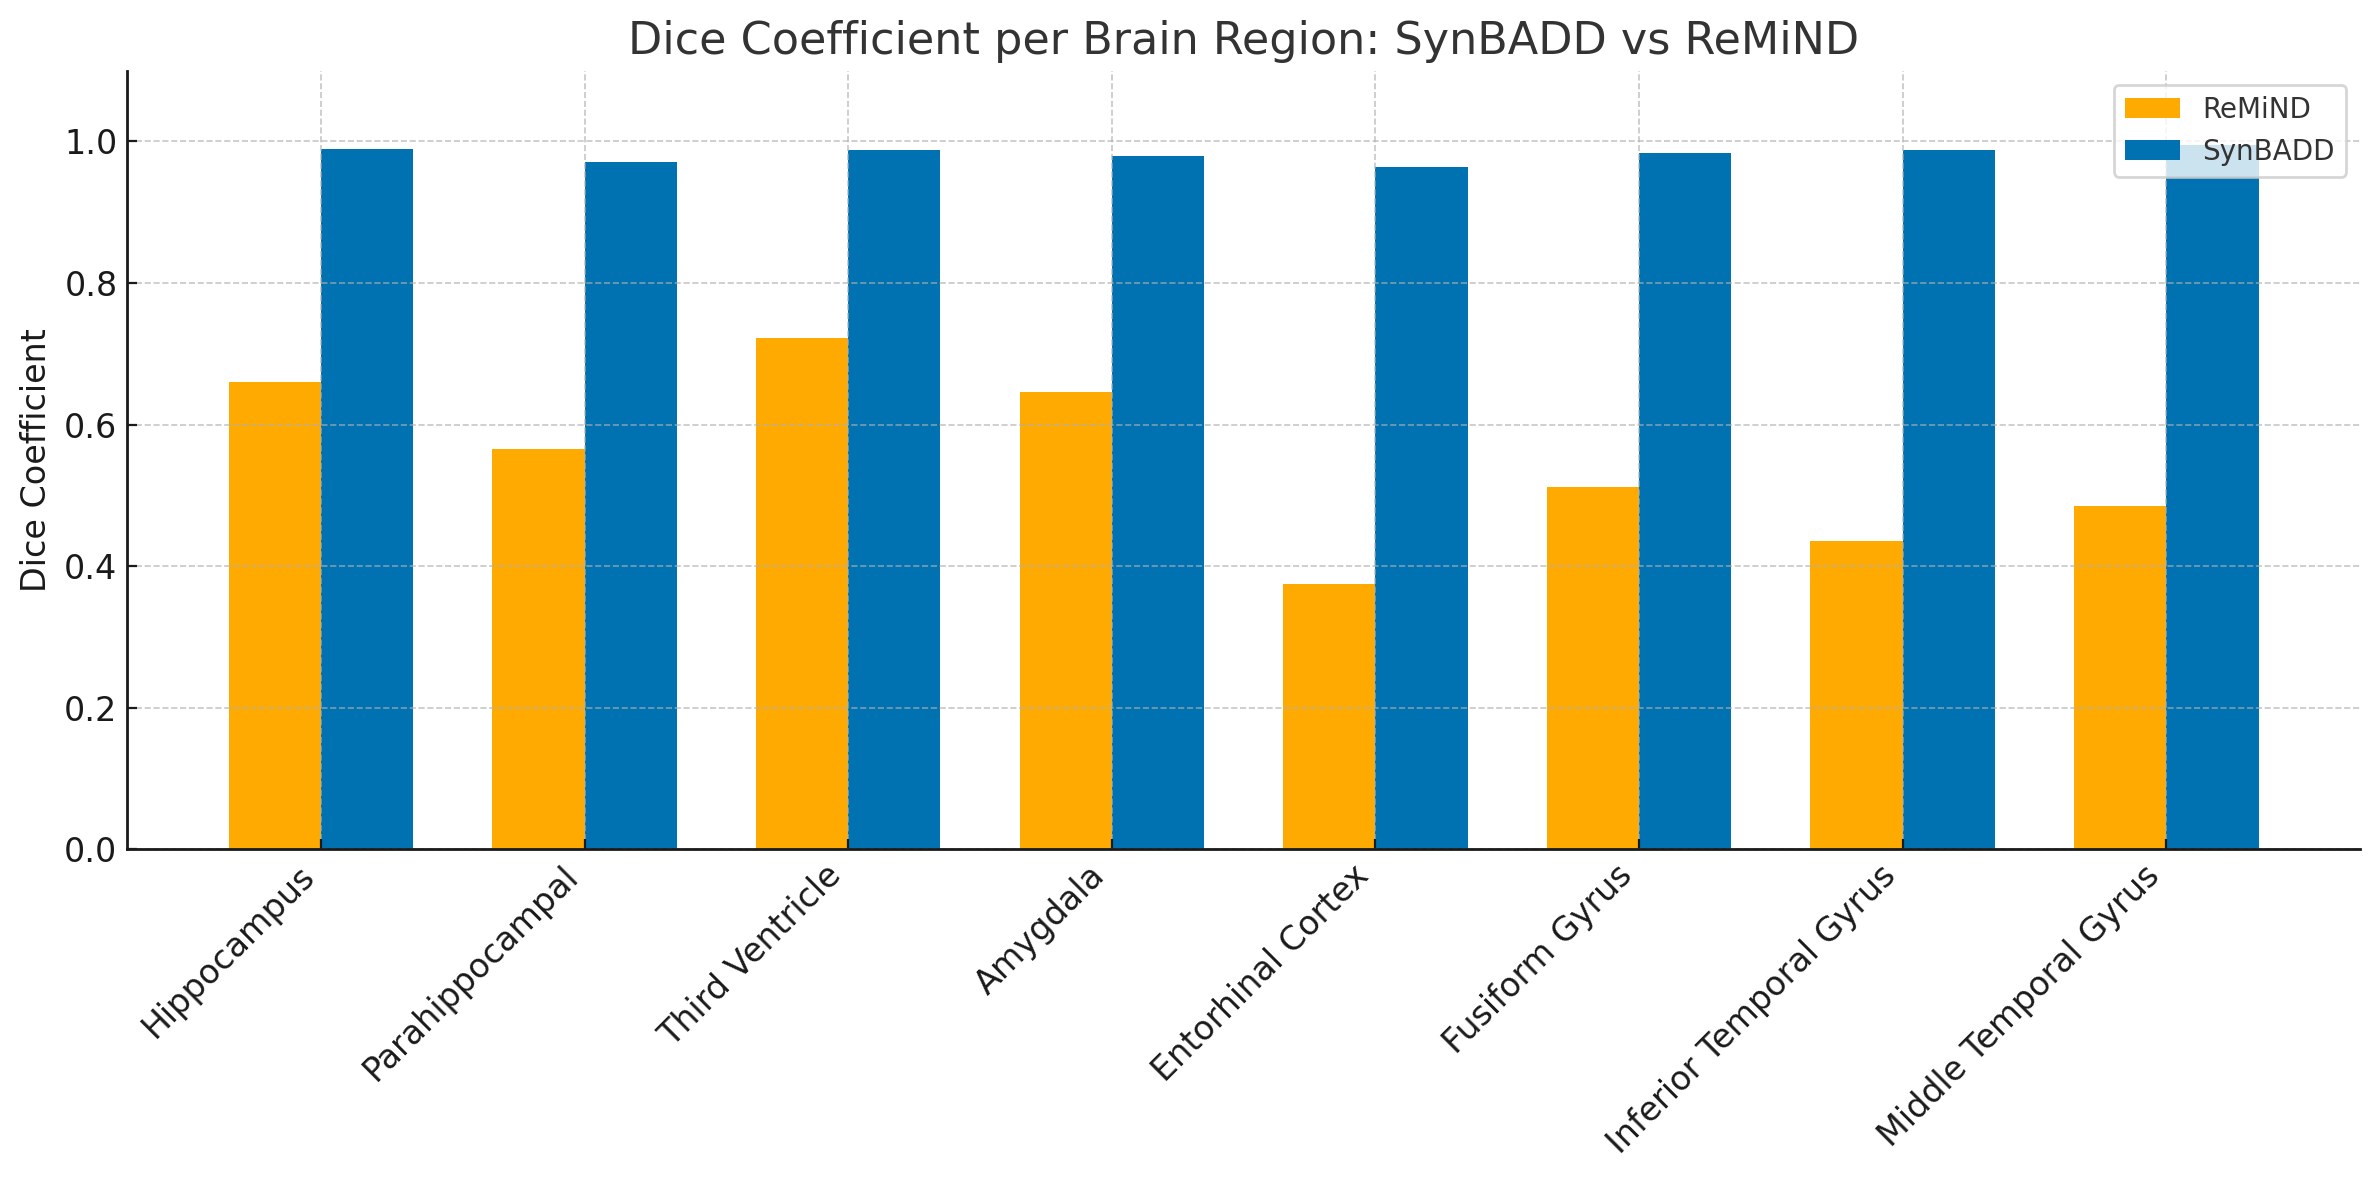
\includegraphics[width=\textwidth]{images/dice synbadd remind.png}
        \caption{Dice coefficient per brain region: SynBADD vs ReMiND.}
        \label{fig:synbadd_remind}
    \end{subfigure}
    \vskip\baselineskip
    \begin{subfigure}[b]{0.8\textwidth}
        \centering
        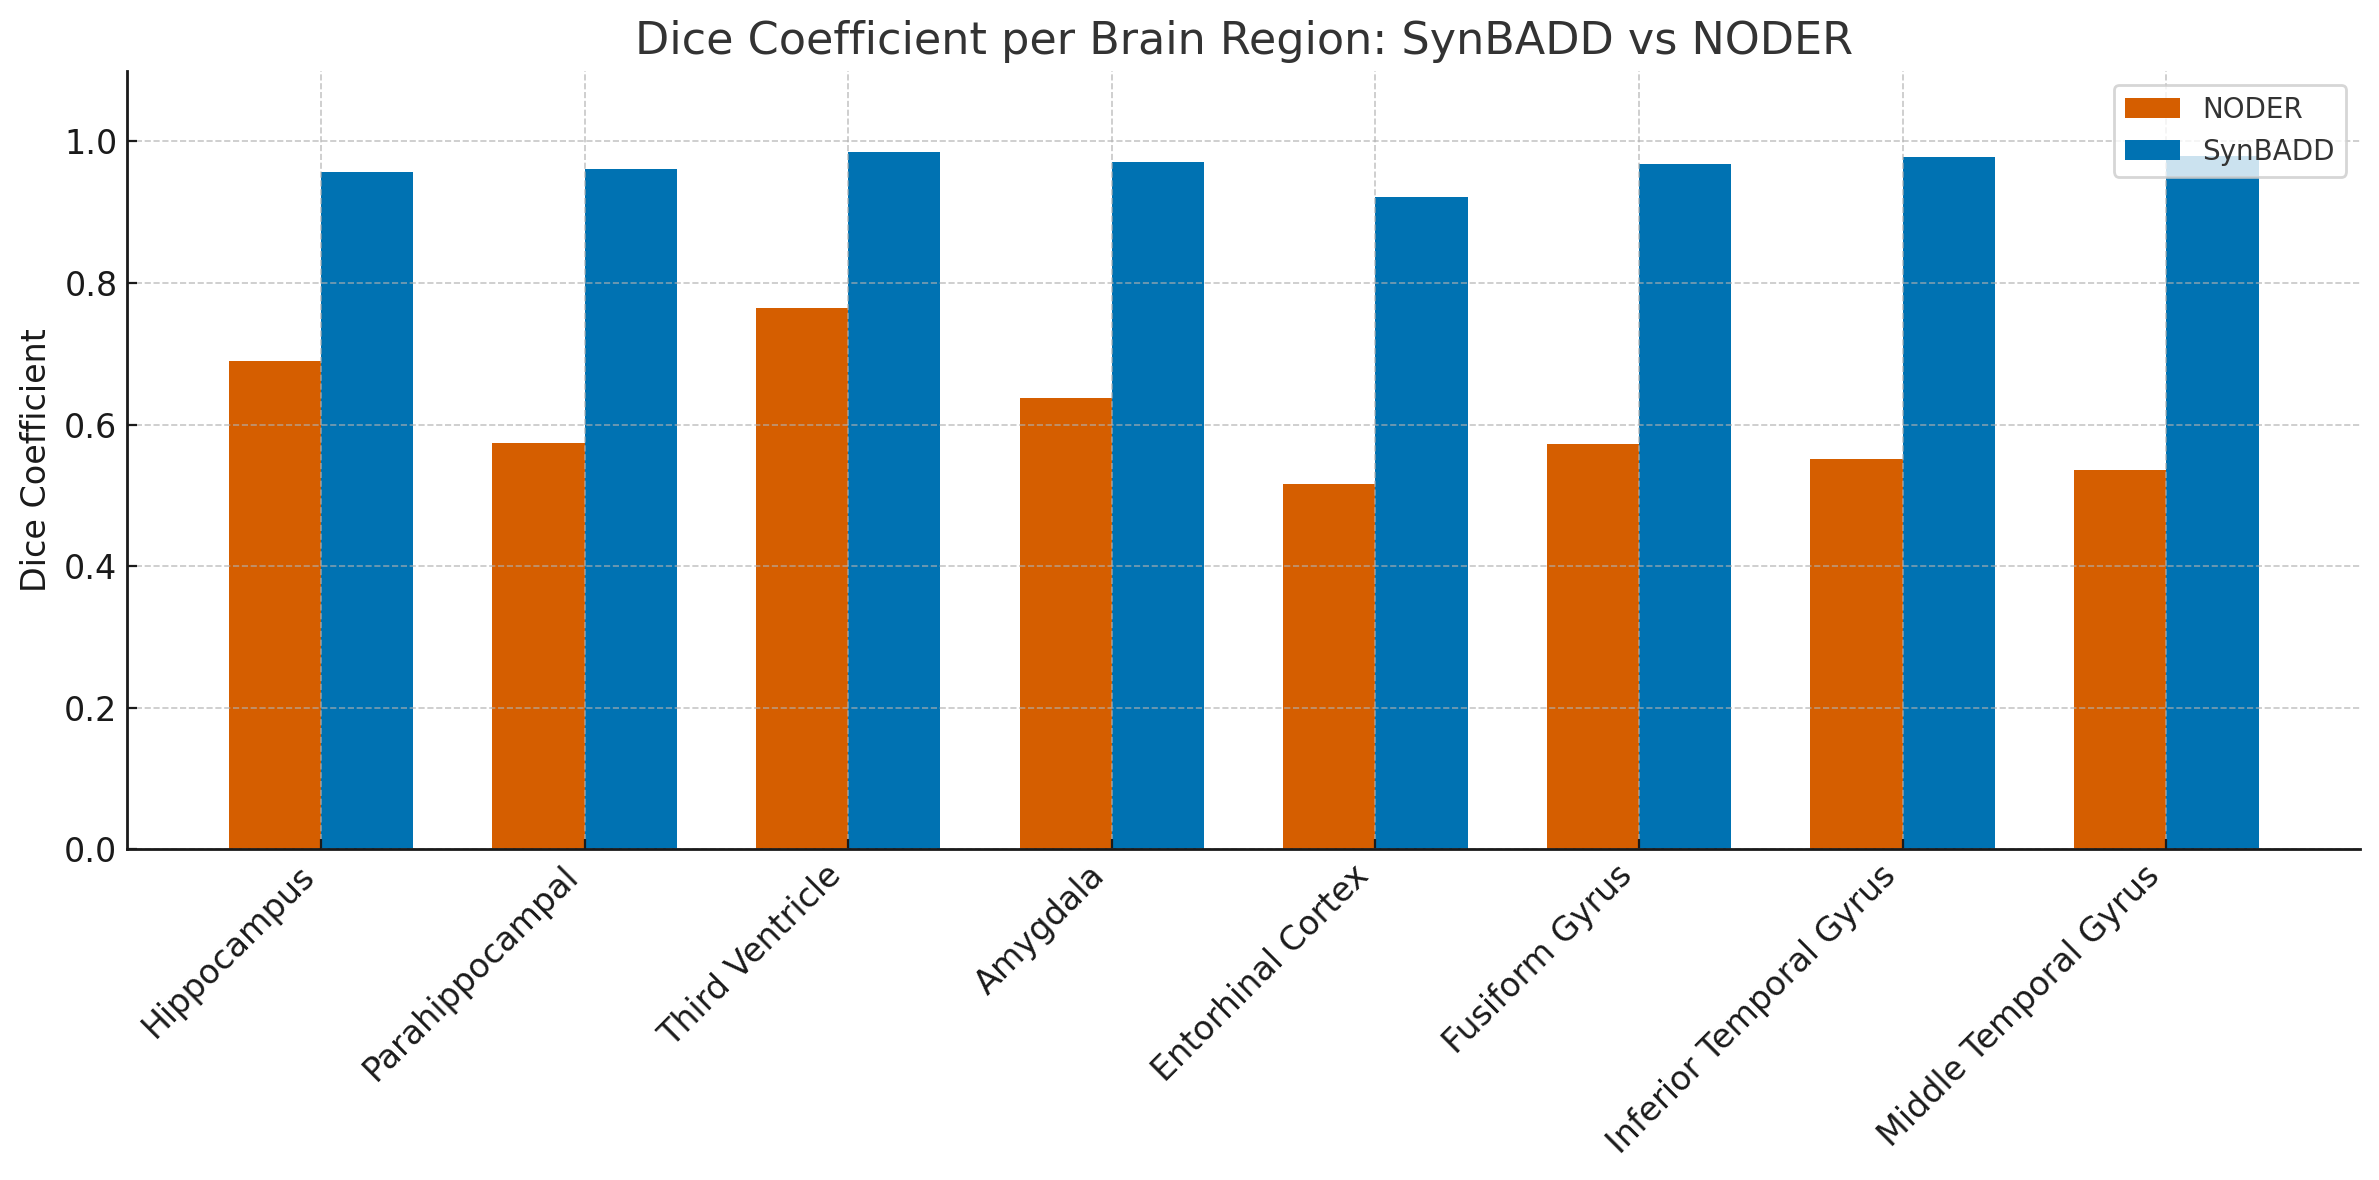
\includegraphics[width=\textwidth]{images/dice synbadd noder.png}
        \caption{Dice coefficient per brain region: SynBADD vs NODER.}
        \label{fig:synbadd_noder}
    \end{subfigure}
    \caption{Dice coefficient comparisons across brain regions between SynBADD, NODER, and ReMiND.}
    \label{fig:comparison}
\end{figure}


% ----------------------------------------------------------
% 5.2.2 Classification of Comparative Methods
% ----------------------------------------------------------
\subsubsection{Classification of Comparative Methods}

To contextualise the performance differences reported above, we characterise each method along several design dimensions that influence imputation quality. These are summarised in Table~\ref{tab:method_taxonomy}.
 
ReMiND operates in the intensity space, generating missing scans by synthesising 2D slices conditioned on the immediately adjacent timepoints. It does not enforce volumetric consistency across slices, nor does it impose explicit anatomical constraints on the generated outputs. Its temporal reasoning is limited to pairwise interpolation between two flanking scans, without access to the broader longitudinal trajectory.
 
NODER models deformations using stationary velocity fields and learns a continuous trajectory in SVF space via neural ordinary differential equations. However, it requires fitting a separate model for each subject and each target timepoint, which limits scalability and introduces susceptibility to overfitting, particularly when the number of available scans per subject is small. Its supervision is based on image regression, which may lead to oversmoothing of predicted deformations.
 
SynBADD shares with NODER the principle of operating in deformation space, but differs in several respects. It trains a single population-level model that generalises across subjects and diagnostic groups, rather than requiring per-subject optimisation. It reasons bidirectionally over the full available longitudinal context, rather than relying on pairwise or unidirectional conditioning. The refinement module, conditioned on clinical metadata, provides subject-specific adaptation within the population-level framework. And the synthesis is performed natively in 3D, producing volumetrically coherent outputs by construction.
 
These design choices collectively account for the observed performance gap. Operating in deformation space preserves anatomical topology, bidirectional attention captures richer temporal context, and population-level training enables robust generalisation even under limited longitudinal sampling.

% ----------------------------------------------------------
% 5.2.2 Quantitative Comparison on Full Evaluation Cohort
% ----------------------------------------------------------
\subsubsection{Quantitative Comparison on Full Evaluation Cohort}

To assess the consistency of the reported improvements, we present per-fold results across all five cross-validation splits. Table~\ref{tab:perfold_psnr} reports PSNR and SSIM for SynBADD and NODER in each fold. SynBADD outperforms NODER in every fold, with per-fold PSNR improvements ranging from 3.07 to 4.13 dB and SSIM improvements ranging from 0.0217 to 0.0268. The variance across folds is small for both methods, confirming that the observed gains are stable and not driven by favourable splits.
 
Table~\ref{tab:perfold_dice} extends this analysis to Dice scores for the hippocampus, parahippocampal gyrus, and third ventricle. SynBADD maintains Dice scores above 0.85 in every fold for all three regions, whereas NODER exhibits greater variability and consistently lower overlap, particularly for the parahippocampal gyrus.
 
We additionally report the Jacobian determinant statistics of the predicted deformation fields in Table~\ref{tab:jacobian}. Across all five folds, SynBADD produces mean Jacobian values in the range of 0.9232--0.9309, with standard deviations of approximately 0.04. A mean Jacobian slightly below unity is consistent with mild tissue contraction, reflecting the predominant atrophy pattern expected in a cohort that includes subjects with MCI and AD. Importantly, no negative Jacobian values were observed, confirming that all predicted deformations are diffeomorphic and topologically valid. This provides additional evidence that SynBADD generates anatomically plausible transformations, not merely transformations that produce visually similar images.

% ----------------------------------------------------------
% 5.2.3 Subgroup Analysis Across Clinical and Temporal Variables
% ----------------------------------------------------------
\subsubsection{Subgroup Analysis Across Clinical and Temporal Variables}

% \textit{[This section will present a disaggregated analysis of SynBADD's performance across clinical subgroups and temporal configurations.]}
 
% \textit{The first part will stratify results by diagnostic group (CN, MCI, AD). We will report PSNR, SSIM, and Dice scores separately for each group to determine whether imputation quality varies with disease severity. This is clinically relevant because subjects with AD exhibit more pronounced and spatially heterogeneous atrophy, which places greater demands on the deformation model. A stable or only mildly degraded performance in the AD subgroup would indicate that SynBADD's deformation-based formulation can accommodate the larger and more localised deformations associated with advanced neurodegeneration.}
 
% \textit{The second part will examine performance as a function of the target timepoint's position within the longitudinal sequence. Missing scans at boundary positions (e.g., the earliest or latest follow-up) have asymmetric temporal context---only past or only future observations are available---whereas centrally positioned missing scans benefit from bidirectional context. Evaluating across timepoint positions will reveal the extent to which the model's performance depends on the availability of flanking observations, and will complement the robustness analysis presented in Section~\ref{sec:robustness}.}
 
% \textit{Tables and figures reporting these disaggregated results will be included upon completion of the subgroup analyses.}


% ----------------------------------------------------------
% 5.3 Robustness to Incomplete Temporal Context
% ----------------------------------------------------------
\subsection{Robustness to Incomplete Temporal Context}
\label{sec:robustness}
 
In clinical practice, subjects rarely present with complete longitudinal imaging sequences. Missed visits, late enrolment, and early dropout frequently result in irregular and sparse temporal sampling. A practical imputation model must therefore degrade gracefully when fewer observations are available, and must handle asymmetric temporal context---where, for instance, more past scans than future scans are accessible, or vice versa. In this section, we evaluate SynBADD's sensitivity to these conditions.

% ----------------------------------------------------------
% 5.3.1 Effect of Reduced Input Timepoints
% ----------------------------------------------------------
\subsubsection{Effect of Reduced Input Timepoints}

% \textit{[This section will evaluate how SynBADD's imputation quality changes as the number of available input timepoints is progressively reduced.]}
 
% \textit{We will construct evaluation scenarios in which the model receives 4, 3, and 2 observed timepoints as context for predicting the missing scan, compared to the full complement of available observations used in the main experiments. For each configuration, we will report PSNR, SSIM, and Dice scores for key regions of interest, averaged over the five cross-validation folds.}
 
% \textit{The expected outcome is a gradual degradation in performance as temporal context is reduced, with the rate of degradation revealing how effectively the transformer leverages partial context. A shallow decline would indicate that the model extracts useful information from even a small number of observations, rather than requiring a densely sampled sequence. This has direct practical implications, as many longitudinal cohorts---including ADNI---contain subjects with only two or three available scans. We will additionally compare the reduced-context performance of SynBADD against the full-context performance of NODER and ReMiND, to assess whether SynBADD under impoverished conditions still matches or exceeds the baselines operating with their standard inputs.}
 
% \textit{A table reporting these results across input counts will be included upon completion of the experiments.}

% ----------------------------------------------------------
% 5.3.2 Effect of Asymmetric Context Availability
% ----------------------------------------------------------
\subsubsection{Effect of Asymmetric Context Availability}

% \textit{[This section will directly test the bidirectional reasoning capability that is central to SynBADD's design, by comparing performance under three temporal context configurations: past-only, future-only, and full bidirectional.]}
 
% \textit{In the past-only setting, the model is given access only to latent codes from timepoints preceding the missing scan. In the future-only setting, only subsequent timepoints are provided. In the bidirectional setting, both past and future observations are available. By comparing these conditions, we aim to quantify the contribution of each temporal direction to the quality of the imputed scan.}
 
% \textit{This analysis is clinically motivated. In many real-world settings, the missing scan corresponds to the most recent follow-up (e.g., a subject who drops out), in which case only past context is available. Conversely, a subject who enrols late may have future scans but lack early observations. Understanding how SynBADD performs under each regime informs its practical applicability and validates the design choice of incorporating bidirectional temporal attention.}
 
% \textit{We anticipate that bidirectional context will yield the best performance overall, but that the model will still produce reasonable imputations under unidirectional conditions, owing to the temporal transformer's ability to attend selectively to whichever context is available. The relative performance drop from bidirectional to each unidirectional setting will quantify the value of each temporal direction. A table comparing PSNR, SSIM, and Dice across the three conditions will be included.}


% ----------------------------------------------------------
% 5.4 Qualitative Analysis of Synthesised Outputs
% ----------------------------------------------------------
\subsection{Qualitative Analysis of Synthesized Outputs}
\label{sec:qualitative}
 
Quantitative metrics capture global image fidelity but may not reveal localised anatomical artifacts or subtle structural inconsistencies that are relevant for clinical interpretation. In this section, we complement the numerical evaluation with qualitative comparisons of synthesised scans across methods, examining both the final warped images and the underlying predicted deformation fields.

% ----------------------------------------------------------
% 5.4.1 Visual Comparison of Predicted Scans
% ----------------------------------------------------------
\subsubsection{Visual Comparison of Predicted Scans}

Figures~\ref{fig:slicewise_1} and~\ref{fig:slicewise_2} present consecutive axial slices (slices 62--66) of synthesised scans for two representative subjects, comparing SynBADD, NODER, and ReMiND against the ground-truth target.
 
ReMiND, which generates each 2D slice independently before stacking them into a volume, exhibits noticeable inter-slice inconsistencies. Intensity discontinuities and hole-like artifacts are visible between adjacent slices, most prominently between slices 63 and 64, where both signal quality and anatomical coherence degrade. These spatial discontinuities compromise the volumetric integrity of the reconstructed scan and would limit its reliability in any downstream analysis that depends on 3D spatial relationships, such as segmentation or morphometric measurement.
 
NODER, as a deformation-based method, maintains volumetric continuity across slices. However, it tends to overestimate local deformations in certain regions, producing protrusion-like artifacts where tissue boundaries are displaced beyond their ground-truth positions. This is consistent with the observation that NODER fits subject-specific trajectories through regression, which can amplify small estimation errors into localised geometric distortions.
 
SynBADD preserves smooth anatomical transitions across all consecutive slices, with no visible discontinuities or exaggerated deformations. The cortical folds, ventricular boundaries, and subcortical structures are consistently rendered across the slice sequence, reflecting the inherent spatial coherence of its 3D deformation-based synthesis.
 
Figure~\ref{fig:diffmaps} presents voxel-wise difference maps between the synthesised and ground-truth scans, displayed as signed error fields in which blue indicates negative intensity differences, red indicates positive differences, and white corresponds to zero error. SynBADD achieves substantially lower error magnitudes across the brain volume compared to both baselines. ReMiND produces widespread errors, particularly in cortical and ventricular regions, reflecting the cumulative effect of slice-wise synthesis artifacts across the volume. NODER shows more localised but pronounced errors along tissue boundaries, consistent with its tendency to overestimate deformation magnitudes. The error distribution of SynBADD is both smaller in magnitude and more spatially uniform, with residual errors concentrated primarily in regions where the ground-truth deformation itself is largest---an expected pattern for a method that models deformation rather than absolute appearance.
 
Figure~\ref{fig:finegrained} provides a detailed view of SynBADD's capacity to capture subtle, localised anatomical changes. In this visualisation, the baseline scan is warped to the target timepoint using the predicted SVF, and the resulting image is compared against both the ground truth and the original baseline. Regions where fine-grained atrophy has been accurately captured by the warping are highlighted, alongside regions where the warped scan diverges from the undeformed baseline. The comparison confirms that SynBADD is sensitive to small but clinically meaningful changes---such as hippocampal volume reduction and ventricular expansion---that are characteristic of early neurodegenerative progression. This sensitivity is a direct consequence of operating in the deformation space, where the model's entire generative capacity is directed toward estimating the transformation rather than reconstructing the full intensity volume from scratch.


% ----------------------------------------------------------
% 5.4.2 Visualization of Predicted Deformation Fields
% ----------------------------------------------------------
\subsubsection{Visualization of Predicted Deformation Fields}

To provide further insight into what the model has learned, we visualise the predicted stationary velocity fields directly. Figure~\ref{fig:svf_vis} displays the SVF for a representative subject, rendered as an RGB-mapped velocity field overlaid on axial, coronal, and sagittal views, where each colour channel encodes the velocity component along one spatial axis and the intensity reflects the local magnitude of the deformation.
 
The predicted deformations are spatially concentrated in regions known to be vulnerable to neurodegeneration in Alzheimer's disease: the medial temporal lobe, hippocampal formation, and periventricular areas. Deformation magnitudes are minimal in stable structures such as the brainstem and cerebellum, which is consistent with the known spatial distribution of AD-related atrophy. This pattern confirms that the model has not learned arbitrary spatial warps, but rather biologically interpretable transformations that reflect the expected progression of neurodegeneration.
 
We additionally examine the Jacobian determinant of the predicted deformation field, which quantifies local volume change at each spatial location. Values below unity indicate tissue contraction, while values above unity indicate expansion. Figure~\ref{fig:jacobian_map} shows the Jacobian determinant map for a representative case, overlaid on the corresponding anatomical slice. Regions of mild contraction (Jacobian values slightly below 1.0) are localised to the hippocampus, parahippocampal gyrus, and temporal cortex, while the ventricular system shows slight expansion---a pattern that is characteristic of progressive brain atrophy and is consistent with the literature on volumetric changes in AD. The absence of negative Jacobian values across the field confirms that the predicted deformation is diffeomorphic, preserving the topology of the underlying anatomy.
 
These qualitative analyses reinforce the quantitative findings and provide interpretable evidence that SynBADD produces not only metrically accurate but also anatomically meaningful and clinically plausible imputations.

% # volume diff as boxplots
% # dice diff as box plots
% # ablation results for each ROI as radar plot
% # target warped color coded field grid warp (no need to show baseline scan)
% # show 1 adni 2 subject, 1 adni 3 subject

% # qualitative eval: baseline, target, warped, jac det

% # forward impute (base) vs sadm vs noder vs remind
%  # mention that dice and volume is not dependent on image resolution or bluriness but the segmentation.

%  # limitations
%  1. only structural imaging, not useful for ad
%  2. discretized time points (mention why regression is bad due to curve fitting objective)
%  % 3. metadata integration of apoe4 etc.
%  4.tissue generation/removal
%  5. non linear trajectories, large sudden deformation which breaks svf constraint like tumor
%  6. small time span, only one dataset -> say we wanted to show a method for missing data imputation where input sequence itself has missing data. we wanted to show a method for modeling a full longitudinal sequence.









% \section{Results and Discussion}

% \subsection{Evaluation of SynBADD Variants}

% \subsubsection{Effect of Temporal Transformer Design}

% show in table \ref{tab:transformer variants}

% \subsubsection{Effect of SVF Refinement}

% shown in the only unet part in table \ref{tab:impact of clinical conditioning}

% \subsubsection{Impact of Clinical Conditioning}

% Shown in Table \ref{tab:impact of clinical conditioning}

% \subsection{Comparison with State-of-the-Art Methods}

% Table \ref{tab:Synbadd_v_Noder} and table \ref{tab:Synbadd_v_Remind}

% As each scan is 128x128x128 and the subject's brain on average only occupies ~50\% of the scan volume, there is a requirement to get rid of noisy components for a fair evaluation across methods. We use brain-masking to extract the brain and compute the metrics on this masked region. NODER and ReMiND were evaluated on separate test sets, with the set for ReMiND being a subset of NODER as ReMiND requires both the immediate succeeding and immediate preceeding scans to be present whereas NODER does not have such a constraint. We benchmark SynBADD in both the scenarios using the same test set as we used for evaluating the other model.

% \begin{table}[ht]
% \centering
% \caption{State-of-the-art (SOTA) benchmarking of our model \textbf{SynBADD} against \textbf{NODER} on image quality metrics. Averaged over 5-fold cross-validation. $\uparrow$ indicates higher is better.}
% \begin{tabular}{>{\bfseries}lcc}
% \toprule
% Metric $\uparrow$ & NODER & SynBADD \\
% \midrule
% PSNR  & 31.40  & 34.52 \\
% SSIM  & 0.9766 & 0.9912 \\
% \bottomrule
% \end{tabular}
% \label{tab:Synbadd_v_Noder}
% \end{table}

% \begin{table}[ht]
% \centering
% \caption{Comparison of our model with and without SVF Refinement (UNET) and with and without clinical conditioning (DAFT). Averaged over 5-fold cross-validation. $\uparrow$ indicates higher is better.}
% \begin{tabular}{>{\bfseries}lcc}
% \toprule
% Metric $\uparrow$ & Only UNet & No Unet+ No DAFT \\
% \midrule
% PSNR  & 33.008994  & 32.3926225 \\
% SSIM  & 0.987614 & 0.9856825 \\
% \bottomrule
% \end{tabular}
% \label{tab:impact of clinical conditioning}
% \end{table}

% \begin{table}[ht]
% \centering
% \caption{Comparison of our model with and without gating. Averaged over 5-fold cross-validation. $\uparrow$ indicates higher is better.}
% \begin{tabular}{>{\bfseries}lccc}
% \toprule
% Metric $\uparrow$ & Cross Attention & Cross Attention + Gating & Gating + Cross Attention \\
% \midrule
% PSNR  & 33.417814  & \textbf{33.4939} & 33.392662 \\
% SSIM  & \textbf{0.988284} & 0.98826 & 0.988202 \\
% \bottomrule
% \end{tabular}
% \label{tab:transformer variants}
% \end{table}

% \begin{table}[ht]
% \centering
% \caption{Dice coefficient comparison between \textbf{SynBADD} and \textbf{NODER} across brain regions. $\uparrow$ indicates higher is better.}
% \begin{tabular}{>{\bfseries}lcc}
% \toprule
% Region & NODER Dice $\uparrow$ & SynBADD Dice $\uparrow$ \\
% \midrule
% Hippocampus             & 0.6898 & \textbf{0.9562} \\
% Parahippocampal         & 0.5742 & \textbf{0.9612} \\
% Third Ventricle         & 0.7647 & \textbf{0.9852} \\
% Amygdala                & 0.6371 & \textbf{0.9705} \\
% Entorhinal Cortex       & 0.5168 & \textbf{0.9209} \\
% Fusiform Gyrus          & 0.5726 & \textbf{0.9679} \\
% Inferior Temporal Gyrus & 0.5512 & \textbf{0.9781} \\
% Middle Temporal Gyrus   & 0.5364 & \textbf{0.9792} \\
% \bottomrule
% \end{tabular}
% \label{tab:Synbadd_v_Noder_dice}
% \end{table}

% Table \ref{tab:Synbadd_v_Remind_dice} shows that \textbf{SynBADD} achieves a Dice improvement in key ROIs relevant for Alzheimer’s disease over \textbf{ReMiND} ranging from $+36.78\%$ for the Third Ventricle to $+157.34\%$ for the Entorhinal Cortex.

% \begin{table}[ht]
% \centering
% \caption{Per-fold PSNR and SSIM results for \textbf{SynBADD} and \textbf{NODER} over 5-fold cross-validation. $\uparrow$ indicates higher is better.}
% \begin{tabular}{>{\bfseries}lcccc}
% \toprule
% Fold & NODER PSNR $\uparrow$ & NODER SSIM $\uparrow$ & SynBADD PSNR $\uparrow$ & SynBADD SSIM $\uparrow$ \\
% \midrule
% Fold 1 & 31.3916 & 0.9766 & 34.3647 & 0.9911 \\
% Fold 2 & 31.4255 & 0.9768 & 35.0268 & 0.9924 \\
% Fold 3 & 31.6984 & 0.9784 & 34.7491 & 0.9917 \\
% Fold 4 & 31.2990 & 0.9744 & 34.0565 & 0.9894 \\
% Fold 5 & 31.1897 & 0.9767 & 34.4068 & 0.9916 \\
% \bottomrule
% \end{tabular}
% \label{tab:Synbadd_v_Noder_detailed}
% \end{table}

% \begin{table}[ht]
% \centering
% \caption{Benchmarking of \textbf{SynBADD} against \textbf{Forward} differences on Volume difference compared to the Ground truth brain regions. Values represent absolute and percentage differences. $\uparrow$ indicates higher is better.}
% \begin{tabular}{>{\bfseries}lcccc}
% \toprule
% Region & Forward Diff & Forward Diff (\%) & SynBADD Diff & SynBADD Diff (\%) \\
% \midrule
% Hippocampus & 561.270 & 10.839 & 108.038 & 1.818 \\
% Parahippocampal & 300.140 & 10.918 & 78.603 & 2.507 \\
% Third\_ventricle & 226.921 & 20.340 & 17.473 & 1.222 \\
% Amygdala & 289.803 & 16.109 & 50.108 & 2.448 \\
% Entorhinal\_cortex & 288.660 & 12.978 & 90.032 & 3.794 \\
% Fusiform\_gyrus & 860.089 & 8.683 & 252.063 & 2.278 \\
% Inferior\_temporal\_gyrus & 1038.476 & 7.305 & 328.559 & 2.094 \\
% Middle\_temporal\_gyrus & 1193.117 & 7.229 & 259.860 & 1.526 \\
% \bottomrule
% \end{tabular}
% \label{tab:Synbadd_v_Forward_diff_volume}
% \end{table}

% \begin{table}[ht]
% \centering
% \caption{Comparison of Dice scores between \textbf{SynBADD} and \textbf{Forward} across brain regions. Values represent average Dice coefficients. Higher is better ($\uparrow$).}
% \begin{tabular}{>{\bfseries}lccc}
% \toprule
% Region & Forward Dice & SynBADD Dice & Dice Diff \\
% \midrule
% Hippocampus & 0.595 & 0.930 & 0.336 \\
% Parahippocampal & 0.437 & 0.903 & 0.466 \\
% Third\_ventricle & 0.598 & 0.973 & 0.376 \\
% Amygdala & 0.582 & 0.916 & 0.334 \\
% Entorhinal\_cortex & 0.471 & 0.855 & 0.384 \\
% Fusiform\_gyrus & 0.432 & 0.864 & 0.432 \\
% Inferior\_temporal\_gyrus & 0.449 & 0.849 & 0.400 \\
% Middle\_temporal\_gyrus & 0.403 & 0.850 & 0.447 \\
% \bottomrule
% \end{tabular}
% \label{tab:Synbadd_v_Forward_diff_dice}
% \end{table}

% \begin{table}[ht]
% \centering
% \caption{Benchmarking of \textbf{SynBADD} against \textbf{ReMiND} on image quality metrics. Results are averaged over 5-fold cross-validation. $\uparrow$ indicates higher is better.}
% \begin{tabular}{>{\bfseries}lcc}
% \toprule
% Metric $\uparrow$ & ReMiND & SynBADD \\
% \midrule
% PSNR  & 24.28  & 33.55 \\
% SSIM  & 0.9511 & 0.9917 \\
% \bottomrule
% \end{tabular}
% \label{tab:Synbadd_v_Remind}
% \end{table}


% \begin{figure}[ht]
%     \centering
%     \begin{subfigure}[b]{0.8\textwidth}
%         \centering
%         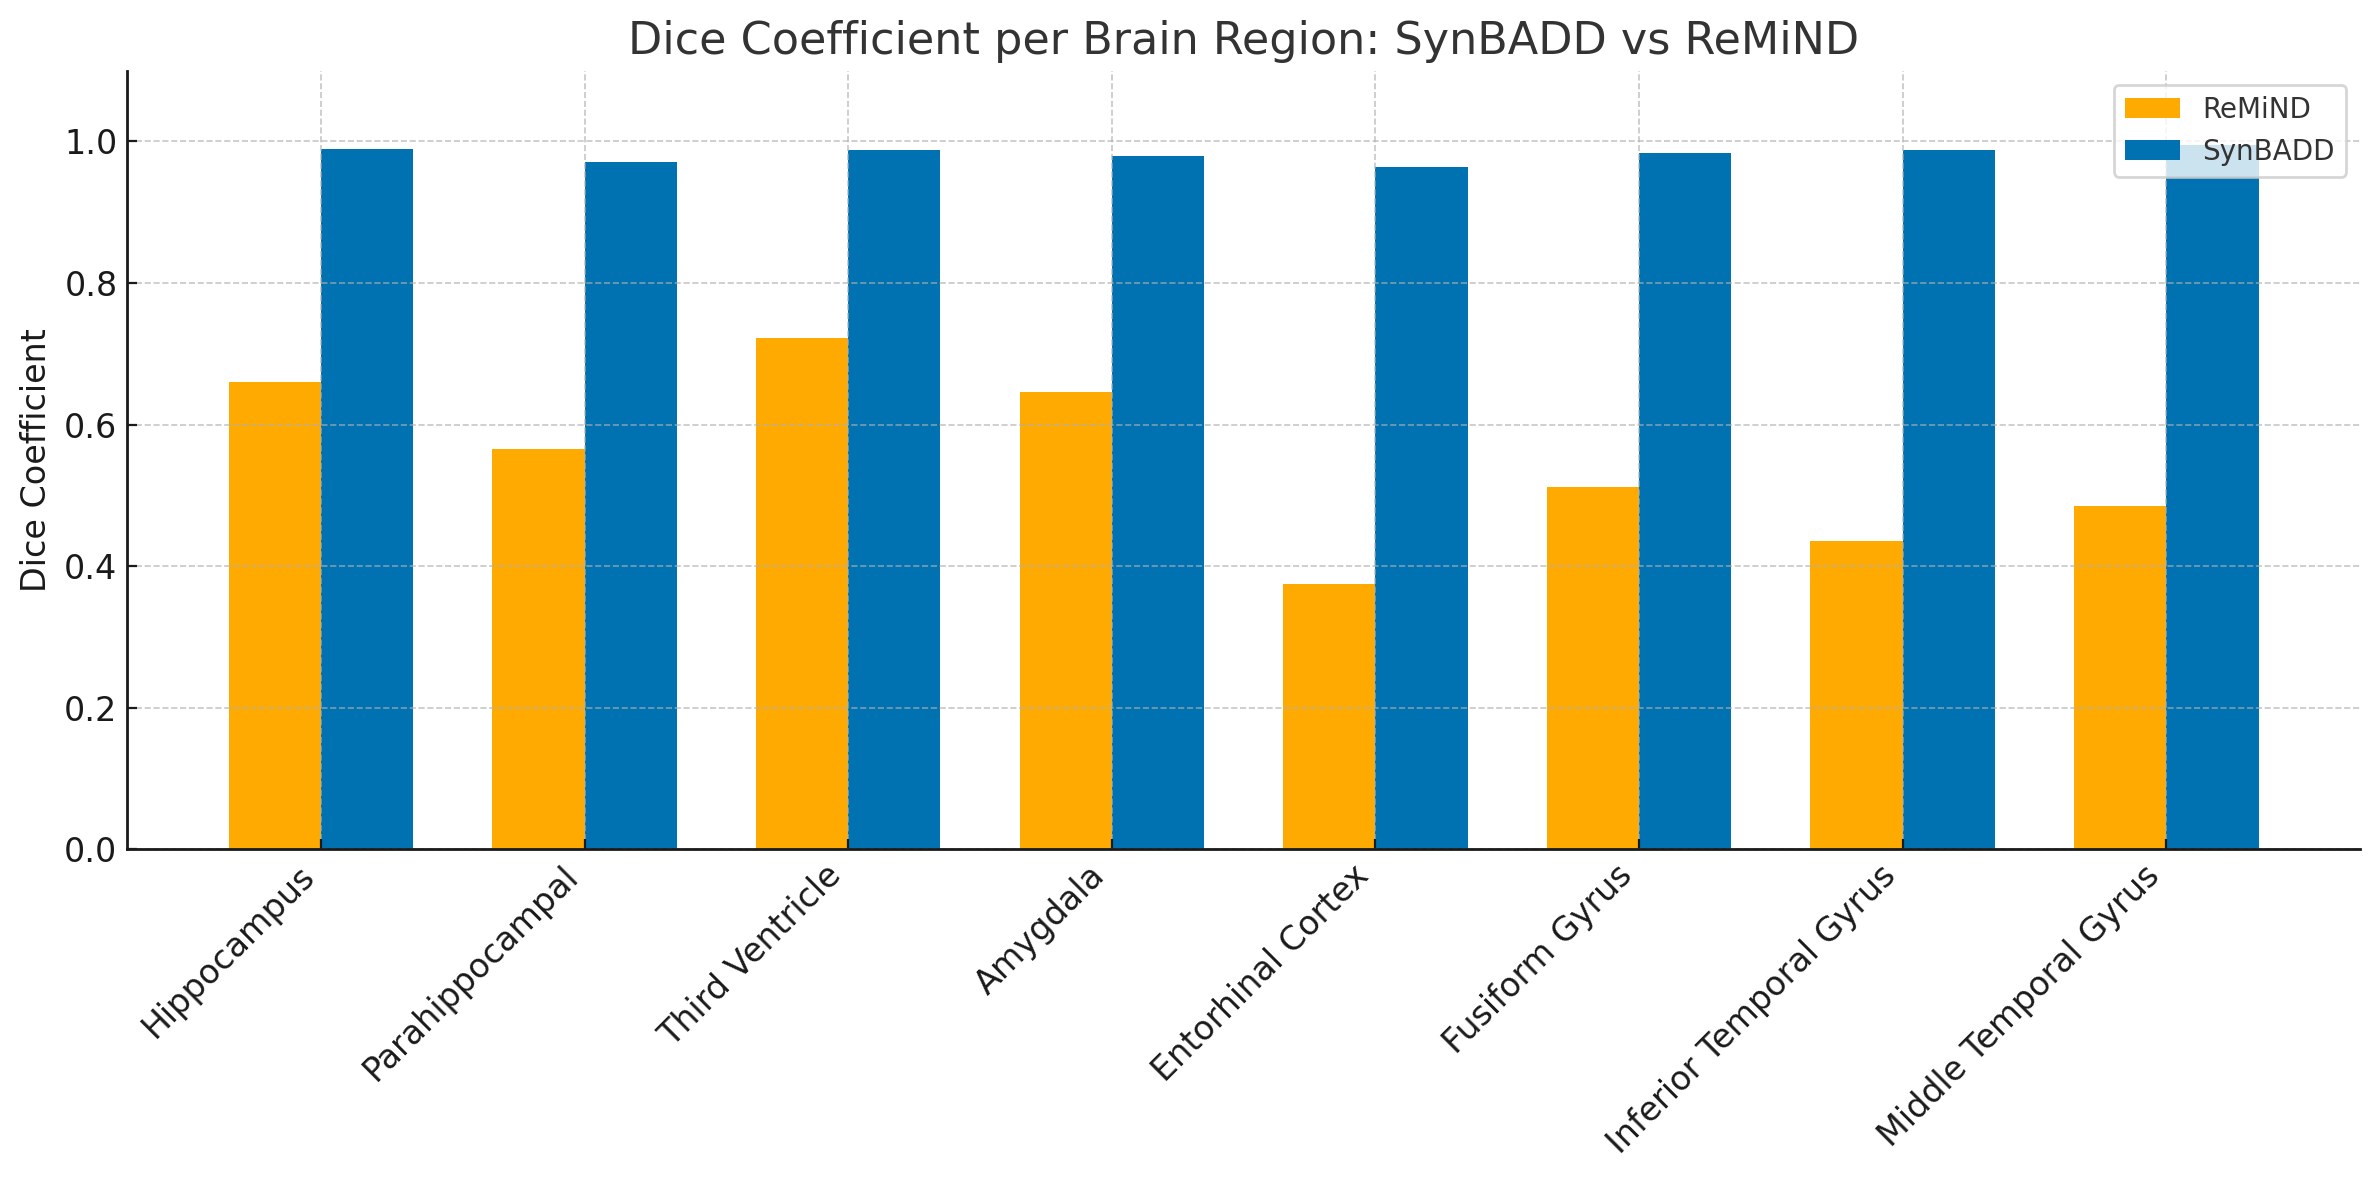
\includegraphics[width=\textwidth]{images/dice synbadd remind.png}
%         \caption{Dice coefficient per brain region: SynBADD vs ReMiND.}
%         \label{fig:synbadd_remind}
%     \end{subfigure}
%     \vskip\baselineskip
%     \begin{subfigure}[b]{0.8\textwidth}
%         \centering
%         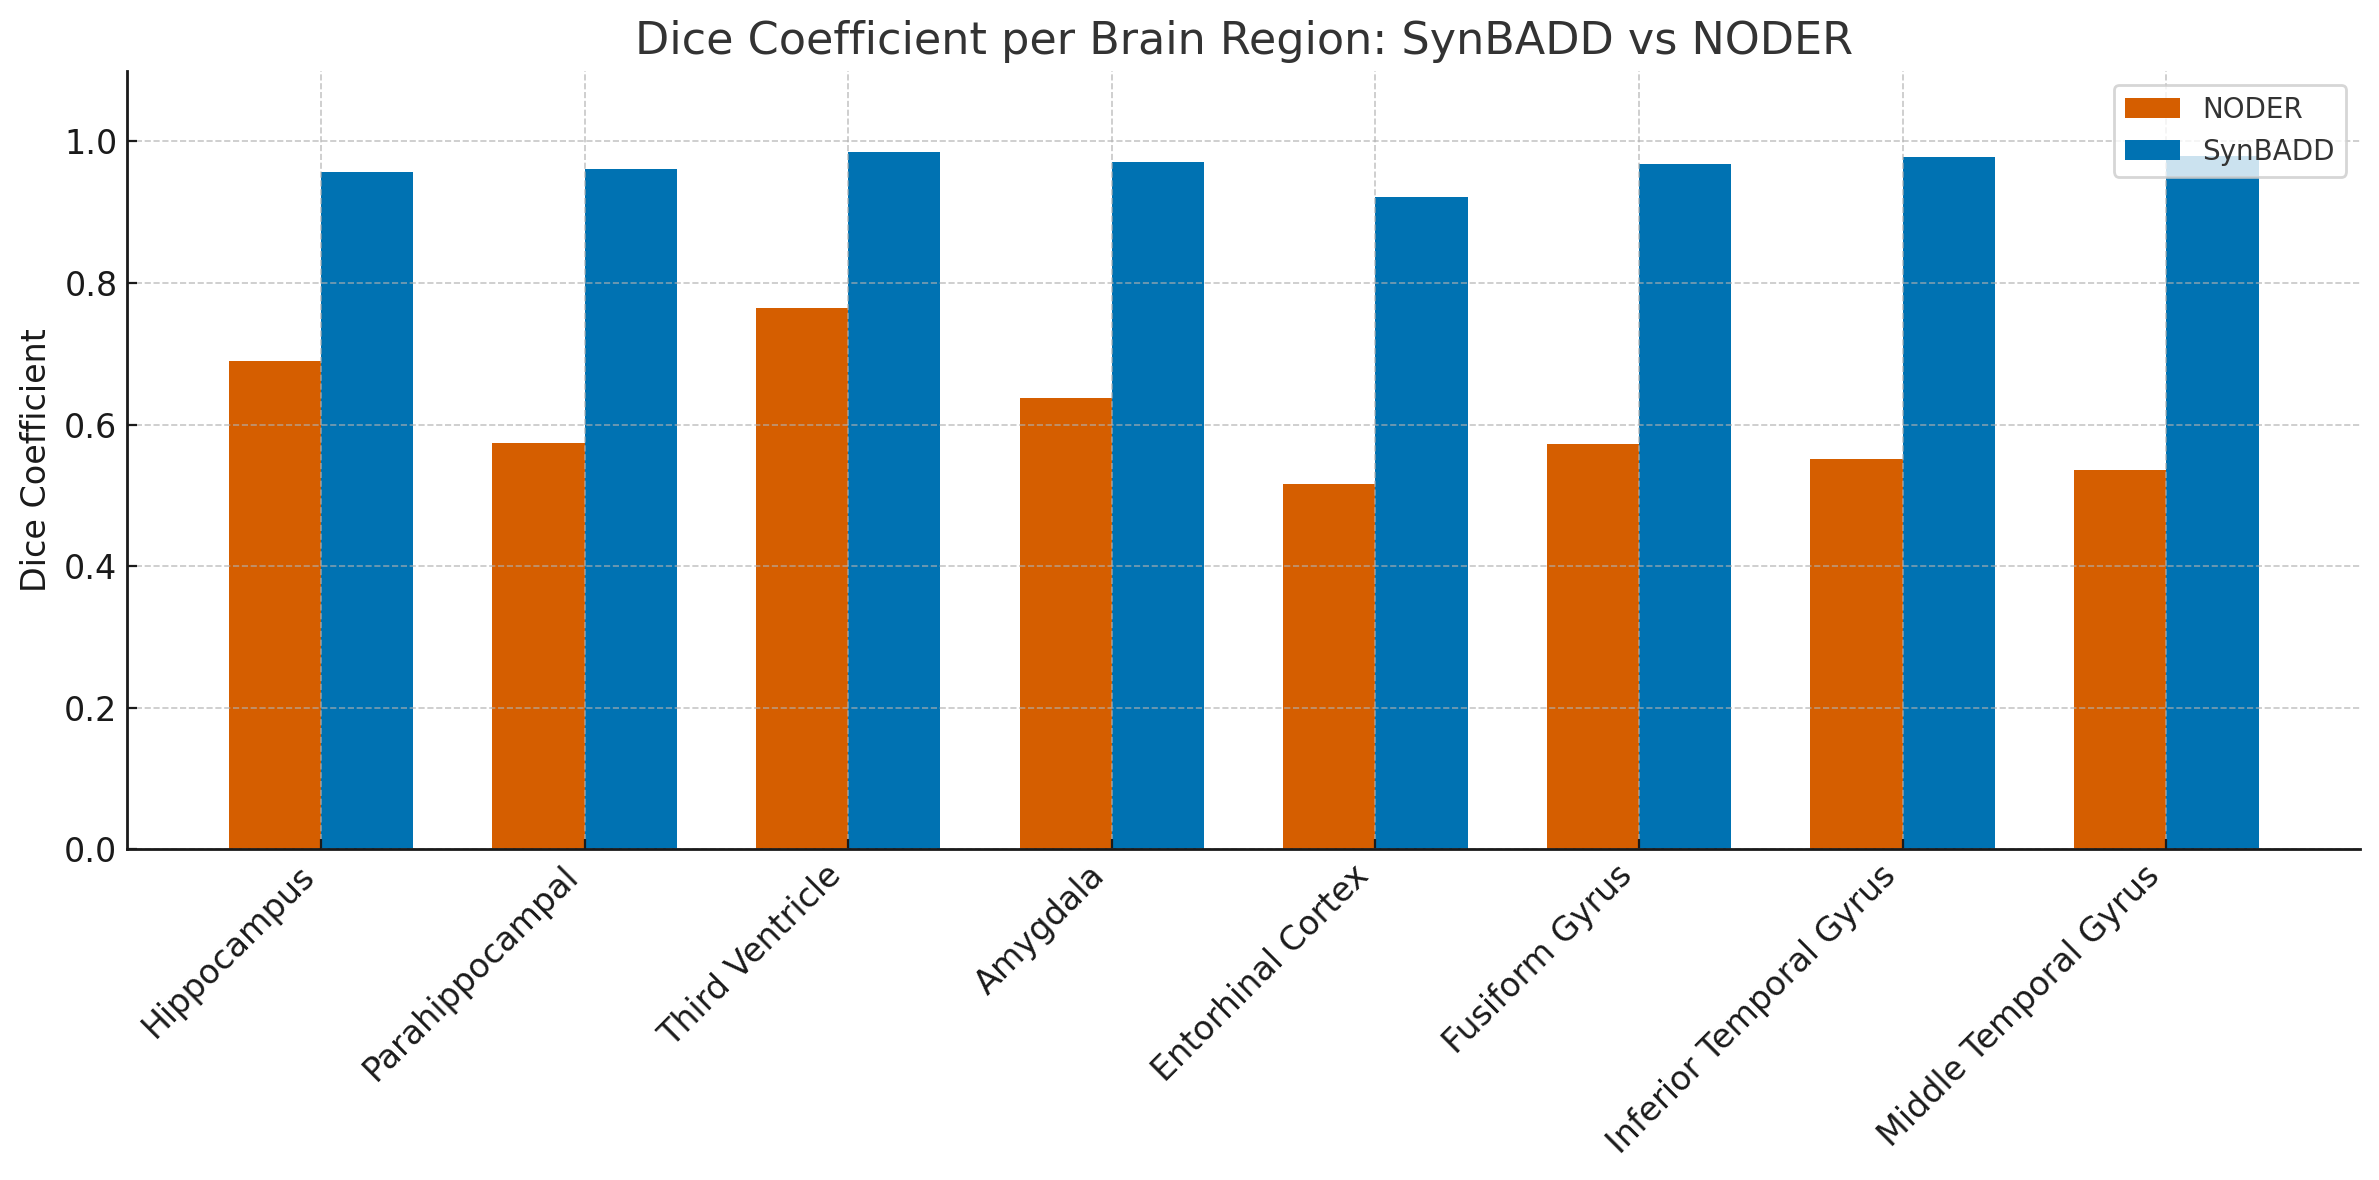
\includegraphics[width=\textwidth]{images/dice synbadd noder.png}
%         \caption{Dice coefficient per brain region: SynBADD vs NODER.}
%         \label{fig:synbadd_noder}
%     \end{subfigure}
%     \caption{Dice coefficient comparisons across brain regions between SynBADD, NODER, and ReMiND.}
%     \label{fig:comparison}
% \end{figure}

% \subsubsection{Classification of Comparative Methods}

% \subsubsection{Quantitative Comparison on Full Evaluation Cohort}

% \subsubsection{Subgroup Analysis Across Clinical and Temporal Variables}

% \subsection{Robustness to Incomplete Temporal Context}

% \subsubsection{Effect of Reduced Input Timepoints}

% \subsubsection{Effect of Asymmetric Context Availability}

% \subsection{Qualitative Analysis of Synthesized Outputs}

% \subsubsection{Visual Comparison of Predicted Scans}

% \subsubsection{Visualization of Predicted Deformation Fields}

% % # volume diff as boxplots
% % # dice diff as box plots
% % # ablation results for each ROI as radar plot
% % # target warped color coded field grid warp (no need to show baseline scan)
% % # show 1 adni 2 subject, 1 adni 3 subject

% % # qualitative eval: baseline, target, warped, jac det

% % # forward impute (base) vs sadm vs noder vs remind
% %  # mention that dice and volume is not dependent on image resolution or bluriness but the segmentation.

% %  # limitations
% %  1. only structural imaging, not useful for ad
% %  2. discretized time points (mention why regression is bad due to curve fitting objective)
% %  % 3. metadata integration of apoe4 etc.
% %  4.tissue generation/removal
% %  5. non linear trajectories, large sudden deformation which breaks svf constraint like tumor
% %  6. small time span, only one dataset -> say we wanted to show a method for missing data imputation where input sequence itself has missing data. we wanted to show a method for modeling a full longitudinal sequence.